    \section{Bias-variance Trade off}
        Ho ho ho! As Christmas is right around the corner, what is more tempting for both student and TA than to read two pages of extra task?! ARE YOU READY?

        We will in the following take a little detour from LWTA neural networks, to investigate an important dissection of model error. The total error of a statistical model can be decomposed into three main contributions; the \textit{bias}, \textit{variance} and \textit{irreducible} error.
        
        Every learning algorithm makes some assumptions about the relationship between the features and target output. Using a model with high bias might result in missing key relations between features and targets, frequently called underfitting. Relaxing model restrictions can yield a lower bias, but at the cost of potentially increasing the variance, often called overfitting. The variance describes how sensitive a model is to fluctuations in training data. High variance might result from a model taking training data noise into consideration when fitting its parameters. Giving the model more constraints can help to decrease the variance, at the cost of introducing more bias. This is the basis for the \textit{bias-variance tradeoff}, where we aim to find the set of parameters where both of these are small. The irreducible error comes from deviation between the assumed underlying function and the targets in the dataset (noise). As the name suggests, this contribution can not be tweaked.  
        \section{Setup and Resampling}
        We will in the following only consider regression problems \footnote{For classification problems, a similar decomposition can be performed, for instance using the \textit{Zero-One loss}, see ~\citep{zero_one_loss}}. In ~\citep{Project1} the bias-variance decomposition for the MSE was derived, giving:
        \begin{align}
            \operatorname{MSE}(\hat{f}) &= \pclosed{\bias(\hat{f})}^2 + \var(\hat{f}) + \sigma^2
        \end{align}
        With $\sigma^2$ as the irreducible error. To estimate model bias and variance, the bootstrap resampling technique will be performed, using a total of 200 bootstrap rounds for each set of model parameters. Taking different sets of models, we will compare between these and try to find the optimal model based minimizing both bias and variance. If not specified otherwise, MSE values (and of course bias and variance) is calculated using the bootstrapped test data.

    \section{Dataset and Preparation}
        The popular video game series FIFA has new releases yearly, with a large fan base for both recreational and competitive play. Consequently, the interest of analyzing in-game data with the goal of getting a small edge is becoming more popular. For instance ~\citep{fifa21playersvalue} tries to estimate players market value based on players characteristics. Here, we will use a similar dataset ~\citep{fifa21_data}, with the goal of calculating the \textit{overall score}, a single number between 1 and 99 representing the players skill and worth. The FIFA21 version will be used. Overall score will be estimated using 38 different minor attributes, such as player dribbling skill and mental composure. All of these are real numbers in the range 1 to 99. In total there are $n = 18944$ players, where we pick a subset of $10000$ players, weighted such that we get players from different football leagues and skill levels. These 38 features are presumably not all FIFA uses to calculate the overall score, indicating that a perfect model can not be found through this approach. 
        
    \section{Umbrella term for methods not neural networks}
        We will present the key theory required for three different sets of estimation methods; \textit{Linear Regression}, \textit{Tree based methods} and \textit{Super Vector Machines}.
        \subsection{Linear Regression}
        For linear regression models, we will consider ordinary least squares (OLS), Ridge regression and Lasso regression. OLS assumes a linear relationship between the features and target, that is a specific data point is simply the sum over features, multiplied by a coefficient for each feature. Ridge and Lasso regression adds a constraint to coefficient sizes, using an $L_2$ and $L_1$ norm respectively, presumably introducing bias. This will be represented through the hyperparameter $\alpha$, proportional to the regularisation strength. See ~\citep{Project1} for a more in depth explanation.
            
        In addition, since all features are assumed to give a positive contribution to the overall score (setting all to 99 should yield an overall score of 99), the coefficients are constrained to be positive.  
        
        \subsection{Tree Based Methods}
            A decision tree uses a flow-chart like structure to generate predictions. Based on a single features value, a \textit{node} performs some test on the feature (i.e. threshold). Using the outcome of the test, the tree follows one of two paths, called \textit{branches}. Each of these branches can then have new nodes, testing based on new features, creating more branches. This continues until no more nodes are reached, where in the regression case, a specific value is predicted. These final outcomes of branches are called \textit{leaves}. The maximum number of nodes, following a single branch, gives the \textit{depth} of the tree. 
            There is a plethora of ways to construct a regression tree. The most common approach is \textit{recursive binary splitting}, where separation of the targets into regions $R_1, R_2, \ldots R_J$ is performed based on the input features. When a simple feature inequality is used, these regions are high-dimensional boxes. Considering the set of features $\set{x_a}$ $a = 1,\ldots,p$. We propose a pair of half-planes 
            \begin{align*}
                R_1(a,s) = \set{X | x_a < s} \text{ and } R_2(a,s) = \set{X | x_a \geq s}
            \end{align*}
            We then aim to find the values of $j$ and $s$ which minimizes
            \begin{align}
                \underset{a,s}{\text{argmin}}\Bigg[ \sum_{y_i \in R_1} (y_i - \bar{y}_{R_1})^2 + \sum_{y_i \in R_2} (y_i - \bar{y}_{R_2})^2 \Bigg] \label{eq:app:tree_optimasation} 
            \end{align}
            Where $\bar{y}_{R_j}$ is the calculated mean of the training data within $R_j$. This is done in a top-down approach, performing the optimasation from \cref{eq:app:tree_optimasation} down each branch, continuing until a stopping criterion is reached. This gives us our regression tree $\hat{f}(x)$, following a specific branch when evaluated for a data point $x_i$. There is no single good measure of model complexity for decision trees, but the depth gives an indication of high finely tuned predictions can become.    

            \subsubsection{Bagged Trees}
            Based on the idea of bootstrap, an ensemble of trees can be constructed. Decision trees are notorious high-variance models which are easily overfitted. By performing bootstrap resampling, a single tree can be fitted for each bag $b$, with the final prediction being the average prediction of each tree.

            \begin{align}
                \hat{F}(x) = \frac{1}{B}\sum_{b = 1}^{B} \hat{f}^b (x) \label{eq:app:bagged_trees}
            \end{align}
            Where $\hat{f}^b$ is a single decision tree, fitted using the data from bag $b$. $B$ represents the total number of trees, which we will call ensemble size.

            \subsubsection{Random Forest}
            Random forest uses the same methodology as bagged trees. Bootstrap is performed in the same manner \cref{eq:app:bagged_trees}, but only a random subset of features is considered at each node split. We represent the number of features considered by $m$, with $m = 1$ reducing to bagged trees. From ~\citep{hastie01statisticallearning}, a ration of $m = \lfloor p/3 \rfloor$ usually performs well on regression problems. This is expedient since trees might be highly correlated, especially if a single feature is highly important for reducing the training MSE. If all features are considered for each split \comment{Not done? -\Anna}
            
            \subsubsection{Boosted trees}
                The idea behind boosted trees is combining several weak learners which iteratively learn from previous mistakes to enhance performance. In the case of decision trees, weak learners are simple trees only performing slightly better than random guesses. 

                When employing gradient boost for regression the process starts by creating a single leaf, with a value $f_0(x)$ often set to the average of all output values in the training set. Implementing a differentiable cost function, e.g. the squared error for regression, the cost of the initial prediction and its gradient with respect to the predicted value is calculated. A simple tree is fitted to minimise the cost. The prediction of that tree is then scaled by a coefficient and is added to the initial prediction, $f_0(x)$, creating the next: $f_1(x) = f_0(x) + \beta b(x;\gamma_1)$. Here $\beta$ is the scaling coefficient and $\gamma_1$ the prediction parameters. The process of calculating the gradient of the cost function, fitting a new tree using the gradient, and adding this tree's prediction to the existing one, is repeated, iteratively creating a better model: 
                \begin{equation}
                    f_M(x) = f_0(x) + \sum_{m=1}^M \beta b(x; \gamma_m)
                \end{equation}
                $\beta$ can be dynamic for various $m$. In that case the gradient of the cost function must also be calculated with respect to $\beta_m$ \citep{hastie01statisticallearning}. 

            \subsection{Support Vector Machines}
            The Support Vector Machine (SVM) is most commonly used in classification problems, with the idea of constricting some hyperplane separating target classes in feature space. By a slight change of approach, the method can also be applied to regression problems, proposed in~\citep{SVR}. 
            
                \subsubsection{Regression Approach}
                    The predictions are performed using a simple linear function
                    \begin{align}
                        f(x_i) = \vec{w}^T x_i + b \text{ with } \vec{w} \in \mathbb{R}^p, b \in \mathbb{R} \label[eq]{eq:SVM_predict} 
                    \end{align}
                    We want to find the optimal values of $\set{\vec{w}, b}$ such that the predictions of $f(x_i)$ lies inside some region around the $y_i$ training data. This region is defined by the hyperparameter $\epsilon$ (the so-called $\epsilon$ intensive tube \footnote{Not to be confused with the famouse $\epsilon$-sausage used for proofs of continuity, introduced by the math professor \textit{Arne Hole}.}). This can be formulated as an optimasation of $\vec{w}$, subject to the $\epsilon$ constraint ~\citep{SVRgood}.  
                    \begin{align}
                        \underset{\vec{w}}{\text{argmin  }}   ||\vec{w}||^2 
                        \hspace{10px}\text{subject to}\hspace{10px} |y_i - f(x_i)| \leq \epsilon \label[eq]{eq:SVM_optimasation}
                    \end{align}
                    This is a so-called \textit{hard margin} approach, where $f(x_i)$ must make a prediction in $[y_i - \epsilon, y_i + \epsilon]$. Relaxations of this constraint can be done, allowing small deviations around the $\epsilon$ tube. This is characterized by the hyperparameter $C \geq 0$, often called a \textit{soft margin}. $C$ is proportional to the margin relaxation (inversely proportional to the regularisation strength), with $C = 0$ reducing to the hard margin approach.  
                
                \subsubsection{Kernels}
                    One of the benefits of SVMs is the magic of the \textit{kernel trick}. Introducing some non-linearity can improve predictions (for instance, see~\citep{Project1} for an example using linear regression). This is done by applying some transformation $\phi$ giving new features in another (often higher dimensional) space $\mathcal{F}$, $\phi: \mathbb{R}^p \xrightarrow{} \mathcal{F}$. For large data sets, especially if $\text{dim}(\mathcal{F}) \gg p$, the transformation complexity can result in long computation times. Luckily, both our model \cref{eq:SVM_predict} and optimasation \cref{eq:SVM_optimasation} only requires the computation of the dot product in $\mathcal{F}$. The kernel trick then gives us a method to calculate the transformed dot product $\phi(x_i)^T \phi(x_i)$, without explicitly calculating $\phi(x_i)$~\citep{kernelTrick}. We express this a function $K(x_i, x_j)$, witch usually some simpler dot product such as $x_i^T x_j$ or $||x_i - x_j||^2$.      
                    \begin{align*}
                        \phi(x_i)^T \phi(x_j) &= K(x_i, x_j)
                    \end{align*}
                    In the following, we will, in addition to the linear (not transformed) product $K(x_i, x_j) = x_i^T x_j$, consider the \textit{Gaussian radial basis function} (RBF) kernel
                    \begin{align}
                        \text{RBF:}\hspace{20px}& K(x_i, x_j) = \text{exp}(-\gamma ||x_i - x_j||)
                    \end{align}
                    Where $\gamma > 0$ is a hyperparameter.
        \begin{figure}[H]
            \centering
            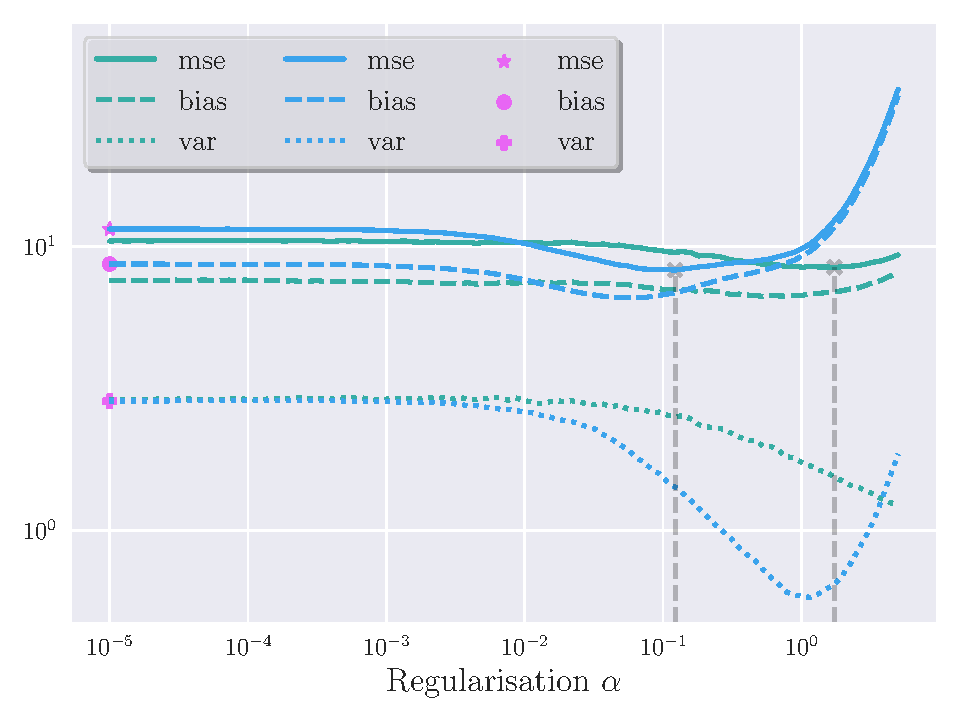
\includegraphics[width=\linewidth]{BiasVar_LinearRegression.pdf}
            \caption{MSE, bias and variance estimates for OLS (pink), Ridge (green) and Lasso (blue) as a function of regularisation parameter $\alpha$.}
            \label[fig]{fig:linreg_biasvar_decomp}
        \end{figure}

        \begin{figure}[H]
            \centering
            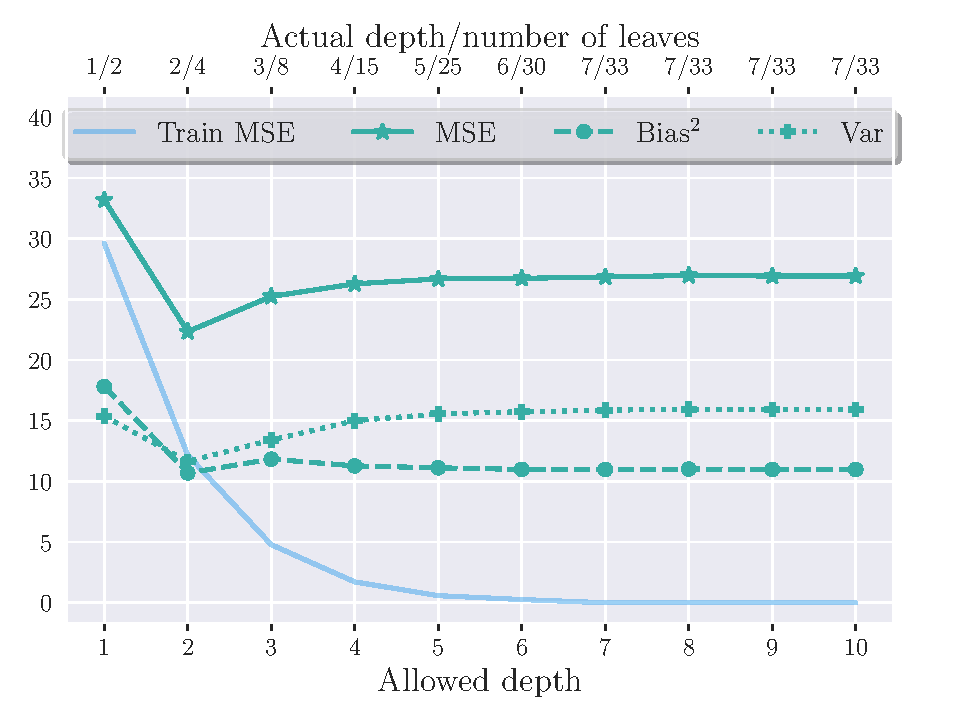
\includegraphics[width=\linewidth]{BiasVar_SingleTree.pdf}
            \caption{MSE, bias and variance estimates for a single tree against increasing relaxation of tree depth.}
            \label[fig]{fig:singletree_biasvar_decomp}
        \end{figure}

        \begin{figure}[H]
            \centering
            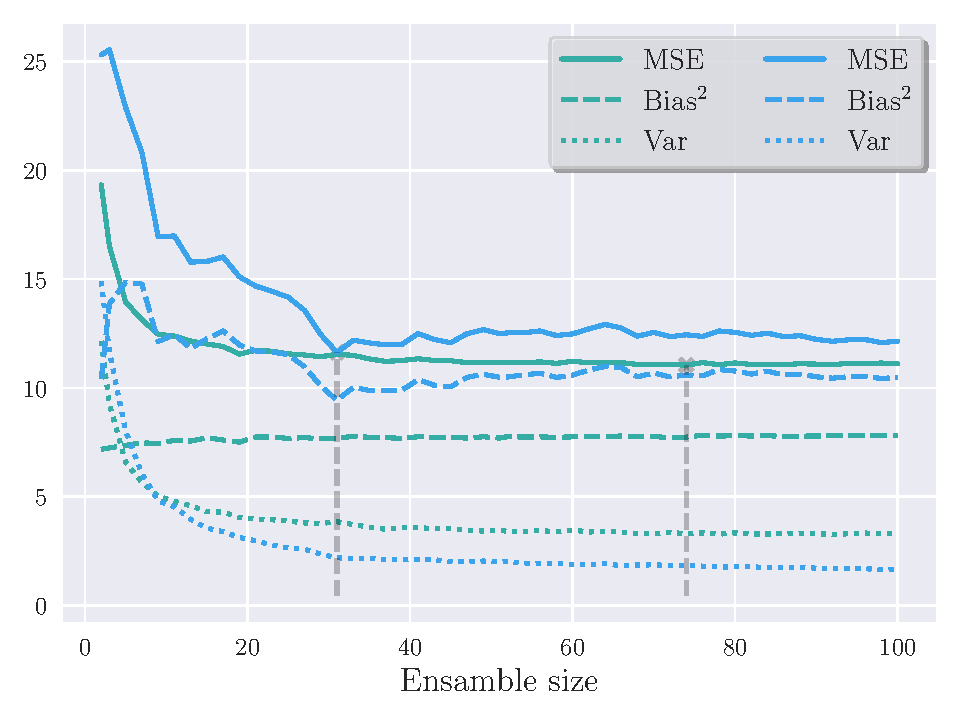
\includegraphics[width=\linewidth]{BiasVar_Bag_and_Rf.pdf}
            \caption{MSE, bias and variance estimates for bagging trees (green) and random forest (blue), against increasing bag size/number of trees.}
            \label[fig]{fig:singletree_biasvar_decomp}
        \end{figure}

